
% ---------------------------
% Lista delle sezioni
% ---------------------------

% - una sezione introduttiva con la descrizione degli algoritmi e delle scelte implementative che avete fatto;
% - grafici esplicativi dei risultati con le risposte alle due domande;
% - eventuali originalità introdotte nell'elaborato o nell'implementazione;
% - una sezione conclusiva in cui porre i vostri commenti e le vostre conclusioni sull’elaborato svolto e i risultati ottenuti.
% - (A PARTE) Il codice sorgente dell’implementazione in un unico file di archivio (.zip, .tar.gz, ecc.).
% Note generali (ultima sezione)


% Start counting pages
\pagenumbering{arabic}
\clearpage
\setcounter{page}{1}

% Introduzione 
\newpage
\section{Introduzione}

\subsection{Descrizione del problema}

In questa relazione illustreremo dei confronti tra tre algoritmi per risolvere un problema
intrattabile, confrontando i tempi di calcolo e la qualità delle soluzioni
che si possono ottenere con \textbf{algoritmi esatti} e con \textbf{algoritmi di approssimazione}.
Il problema in questione è il \textbf{Travelling Salesman Problem} (\textbf{TSP} o
\textit{Problema del Commesso Viaggiatore}). Il nome di questo problema deriva dalla sua
definizione: data una rete di città, connesse tra loro tramite strade, si determini il
percorso di minore distanza che un commesso viaggiatore deve fare per visitare tutte le città
\underline{una e una sola volta}.

Il \textit{TSP} si può rappresentare con un grafo non orientato, pesato e
completo $G = (V,E)$, dove i vertici sono le città e il peso del lato $(u,v)$
è uguale alla distanza da $u$ a $v$. Risolvere il \textit{TSP} significa trovare un
\textbf{circuito Hamiltoniano}, ovvero un ciclo di costo minimo che visita tutti
i vertici \textit{esattamente una volta}.

\subsection{NP-completezza del problema}

\subsubsection{Dimostrazione di NP-completezza}

Prima di tutto dimostriamo che TSP $\in \mathcal{NP}$. Data un'istanza del problema, usiamo
come \textit{certificato} la sequenza degli $n$ vertici del ciclo di peso minimo.
L'algoritmo di verifica del certificato deve controllare che la sequenza contenga ogni
vertice di $G$ esattamente una volta, sommare il peso dei lati e controllare che il peso
totale del ciclo sia inferiore a $k$. Questo controllo si può svolgere in tempo polinomiale
($O(n)$).

Per poter stabilire con precisione la complessità del problema, è necessario prima
“trasformare” tale problema in un \textit{problema di decisione}, aggiungendo un limite $k$
per il peso del ciclo all'input del problema.

\textbf{Definizione di TSP decisionale}: Dato un grafo non orientato, completo e pesato
$G = (V,E)$ e un valore $k > 0$, esiste un ciclo in $G$ che attraversa tutti i vertici una
sola volta di peso inferiore a $k$.

\textbf{Teorema}: \textit{TSP} è un problema $\mathcal{NP}$-completo.

\textit{Dimostrazione}: è già stato dimostrato che \textit{TSP} $\in \mathcal{NP}$, quindi si procede nel dimostrare
che \textit{TSP} è $\mathcal{NP}$-hard. Si mostra quindi una riduzione del problema del circuito Hamiltoniano a TSP.
Prendiamo un grafo non orientato $G = (V,E)$ e costruiamo un'istanza di \textit{TSP} che ci permetta di risolvere
il problema del circuito Hamiltoniano su $G$. Costruiamo un grafo non orientato e completo $G' = (V, E')$
con gli stessi vertici di $G$ e $E' = \{(u, v) | u, v \in V\}$. Il peso degli archi di $G'$ viene assegnato
come segue

\[
    w(u, v) = 0, \textnormal{ se } \{u, v\} \in E
\]
\[
    w(u, v) = 1, \textnormal{ se } \{u, v\} \notin E
\]

È possibile notare che si può costruire il grafo $G'$ in tempo polinomiale rispetto al numero
di vertici $|V|$ del grafo di partenza $G$. Il grafo $G$ contiene un circuito Hamiltoniano se e
solo se $G'$ ha un ciclo di peso minore o uguale a 0. Supponiamo che $G$ contenga un circuito
Hamiltoniano $h = v_1, \dots, v_n$. Ogni lato che compone $h$ è presente in $E$ e quindi ha peso 0 in $G'$.
Di conseguenza, $h$ è un ciclo di $G'$ di peso uguale a 0. Viceversa, supponiamo che $G'$ contenga un ciclo
semplice $t$ che attraversa tutti i vertici di peso minore o uguale a 0. Poiché i pesi dei lati
in $G'$ sono solo 0 oppure 1, tutti i lati che compongono $t$ devono avere costo 0. Quindi tutti i
lati del ciclo sono presenti anche in $E$ e $t$ è un circuito Hamiltoniano per $G$. $ \square $

\subsubsection{Inapprossimabilità per fattori $\rho$ costanti di TSP}

Il \textit{TSP} è un problema simile al problema del MST: il MST è un cammino di peso minimo
che collega tutti i vertici del grafo $G$, mentre il \textit{TSP} è un ciclo di peso minimo
che collega tutti i vertici del grafo $G$. Nonostante questa somiglianza tra questi
due problemi, il \textit{TSP} è un problema molto difficile anche solo da approssimare. Se
esistesse un algoritmo di approssimazione con un $\rho$ costante, allora si saprebbe
risolvere in tempo polinomiale un problema \textit{$\mathcal{NP}$-hard}.

\textbf{Teorema}: se $\mathcal{P} \ne \mathcal{NP}$, non può esistere alcun algoritmo
(polinomiale) di $\rho$-approssimazione per \textit{TSP} con $\rho = \mathcal{O}(1)$.

\textit{Dimostrazione}: per assurdo, si supponga che esista un algoritmo $A_\rho$
polinomiale di $\rho$-approssimazione per \textit{TSP}. Si dimostra come costruire $A_{Hamilton}$
che decide il problema del ciclo Hamiltoniano in tempo polinomiale. Sia $I = G =(V,E)$
e $O = $ "$G$ contiene un ciclo Hamiltoniano?". Si effettua quindi una \textit{riduzione}:
\[
    G \rightarrow G' = (V, E') \textnormal{ è completo, dove }
\]
\[
    c(e \in E') = 1 \textnormal{ se } e \in E \textnormal{, altrimenti } c(e \in E') = \rho|V| + 1
\]

Possiamo quindi creare delle rappresentazioni di $G'$ e di $c$ a partire dalle rappresentazioni
di $G$ in tempo polinomiale in $|V|$ ed $|E|$.

Eseguo $A_\rho(G') \rightarrow C \textnormal{ (ciclo), } c(C) \textnormal{(funzione di costo di $C$, $c: V \times V \rightarrow \mathcal{N}$)}$ e si
determina:
\begin{enumerate}
\item $G \in HAMILTON \Rightarrow c(C^*) = |V| \Rightarrow A_\rho$, ritorna un ciclo $C$
con $c(C) \le \rho|V|$;
\item $G \not\in HAMILTON \Rightarrow C$ contiene almeno un lato non in
$G$ (più precisamente in $E$) $\Rightarrow c(C) \ge \rho|V| + 1$. Poiché i lati che non
appartengono a $G$ sono costosi, c'è un \textit{gap} di almeno $\rho |V|$ tra il costo di un cammino
che è Hamiltoniano in $G$ (di costo $|V|$) e il costo di qualsiasi altro cammino (di costo
almeno $\rho |V| + |V|$). Pertanto, il costo di un cammino che non è un ciclo Hamiltoniano
in $G$ è almeno un fattore $\rho + 1$ maggiore del costo di un cammino che è un ciclo
Hamiltoniano in $G$.
\end{enumerate}

È possibile notare che si può costruire il grafo $G'$ in tempo polinomiale rispetto al numero
di vertici $|V|$ del grafo di partenza $G$. Il grafo $G$ contiene un circuito Hamiltoniano se e
solo se $G'$ ha un ciclo di peso minore o uguale a 0. Supponiamo che $G$ contenga un circuito
Hamiltoniano $h = v_1, ..., v_n$. Ogni lato che compone $h$ è presente in $E$ e quindi ha peso 0 in $G'$.
Di conseguenza, $h$ è un ciclo di $G'$ di peso uguale a 0. Viceversa, supponiamo che $G'$ contenga un ciclo
semplice $t$ che attraversa tutti i vertici e di peso minore o uguale a 0. Poiché i pesi dei lati
in $G'$ sono solo 0 oppure 1, tutti i lati che compongono $t$ devono avere costo 0. Quindi tutti i
lati del ciclo sono presenti anche in $E$ e $t$ è un circuito Hamiltoniano per $G$. $\square$

\label{tsp_metrico}
\subsection{TSP metrico}

Istanza particolare \textit{TSP} in cui l'input, in particolare la funzione di costo $c$, soddisfa la
\textbf{disuguaglianza triangolare}:
\[
\forall u, v, w \in V, \textnormal{ vale che } c(u, v) \le c(u, w) + c(w, v) \Rightarrow
c(<u, v>) \le c(<u, w, v>)
\]

dove $c$ è la \textit{funzione di costo}. Secondo questa definizione, per ogni insieme di tre nodi
possibili del grafo $G$, vale che il costo di un lato $(u, v)$ è al più il costo di un lato $(u, w)$
più il costo di un lato $(w, v)$. Questo significa che il costo del cammino per andare da $u$ a $v$
attraverso l'unico lato che li collega è più conveniente del cammino per andare da $u$ a $w$ e da
$w$ a $v$. Chiamiamo questo problema \textbf{TRIANGLE\_TSP}. Questa restrizione del problema
$\mathcal{NP}$-completo si trova in $\mathcal{P}$.

% \textbf{Teorema}: 

% Descrizione degli algoritmi
\section{Descrizione degli algoritmi}

\subsection{Struttura dati per il grafo}

La struttura dati per il grafo è stata implementata nel seguente
modo:
\begin{enumerate}
    \item \verb|V| è un insime di nodi;
    \item \verb|E| è una lista di lati;
    \item \verb|graph| rappresenta la \textit{lista di adiacenza}.
    Gli indici per accedere alla mappa sono rappresentati dai vertici.
    Ogni cella della mappa punta ad una lista di coppie di valori
    (il vertice a cui è collegato e il peso del lato che li
    congiunge).
\end{enumerate}

I metodi implementati sono:
\begin{enumerate}
    \item \verb|add_vertex|: aggiunge un vertice al grafo;
    \item \verb|add_edge|: aggiunge un lato al grafo;
    \item \verb|remove_edge|: rimuove un lato dal grafo.
\end{enumerate}
Queste operazioni sono state implementate in modo da avere una
complessità computazionale costante.

\subsection{Kruskal naive}

\subsubsection{Introduzione}

La versione naive dell'algoritmo di Kruskal ha una complessità
computazionale pari a $O(mn)$. L'idea alla base di questo
algoritmo è quella di ordinare i lati in ordine crescente rispetto al
loro peso $w$. Una volta ordinati, per ogni lato si controlla se
aggiungendolo al grafo temporaneo questo crei un ciclo. Se crea un
ciclo allora tale lato non verrà inserito, altrimenti il lato farà
parte dell'MST $T$.

Ordinando i lati in base al loro peso e controllando che l'inserimento
di un lato non crei un ciclo nel grafo, si otterà un albero la cui
somma dei suoi lati sarà minima.

Si illustri lo pseudo-codice:
\begin{verbatim}
    Kruskal-Naive(G)
        A = Graph()
        for each vertex v in G.V
            G.add_vertex(v)
        sort the edges of G.E into increasing order by weight w
        for each edge (u, v) in G.E, taken in increasing order by weight
            if A U {(u, v)} is acyclic
                A = A U {(u, v)}
        return A
\end{verbatim}

\subsubsection{Implementazione}

Nella nostra implementazione, abbiamo utilizzato l'algorimo di
ordinamento \textit{merge sort}, che cha una complessità
computazionale pari a $\Theta(n log(n))$, per ordinare i lati
in ordine crescente rispetto al loro peso.

Il Minimum Spanning Tree viene salvato in una struttura dati
\verb|Graph|. Il MST può essere esaminato andando ad
esplorare la lista di adiacenza \verb|graph| o la lista dei
lati \verb|E|.

Il controllo per la ciclicità viene implementato con una
versione modificata della \textit{Depth First Search}
(\textit{DFS}).

\subsubsection{Ottimizzazioni implementate}

Per ottimizzare l'algoritmo abbiamo apportato delle opportune
modifiche. A partire dal metodo \verb|kruskal_naive|, ad
ogni iterazione del ciclo, si controlla se il numero di lati
del grafo $A$ (quello che conterrà il MST) ha $n - 1$ lati,
dove $n$ è il numero di vertici del grafo $G$, fornito in input.
Quando si raggiunge questa uguaglianza, significa che è stato
costruito il MST $T$, pertanto l'algoritmo può terminare.
Questa prima modifica permette di evitare di fare iterazioni
inutili che non contribuiranno alla costruzione del MST.

La seconda ottimizzazione implementata riguarda il metodo
\verb|_is_acyclic|. Un primo controllo riguarda i vertici
connessi dal lato. Se i due vertici sono uguali significa
che il lato in questione crea un \textit{self-loop}. Con
questo controllo siamo in grado eliminare i self-loop in
tempo costante, senza dover effettuare una chiamata a DFS per verificare
che l'aggiunta di tale lato crei un ciclo nel grafo $A$.
Il secondo controllo che è stato implementato in questo metodo
riguarda i vertici $u$ e $v$ che il lato, fornito in input, connette.
Se almeno uno dei due lati non è presente nel grafo $A$, allora
possiamo concludere che tale lato non introdurrà un ciclo nel grafo,
in quanto il lato in questione permetterà di scoprire almeno un nuovo
vertice del MST finale. Questa accortezza ci permette di risparmiare
di effettuare delle chiamate a DFS soprattuto nella fase di avvio
dell'algoritmo. Se invece, sia $u$ che $v$ sono già presenti
nel grafo $A$, allora è necessario fare una chiamata a DFS per verificare
che quel lato non introduca un ciclo nel grafo.

La terza ottimizzazione riguarda DFS. Il metodo che è stato implementato
non rispecchia la versione originale dell'algoritmo. Lo scopo di DFS
è quello di andare a visitare \textit{tutti} i vertici di un certo
grafo. Tuttavia, questo non rappresenta il nostro scopo. Il nostro
intento è quello di cercare, se esiste, un cammino che congiunge $u$ con
$v$. Se tali vertici si trovano in due componenti connesse distinte
(può capitare nel momento in cui si stanno aggiungendo i lati al
grafo $A$), significa che l'aggiunta del lato $(u, v)$ al grafo $A$ non
introdurrà un ciclo. Avviando DFS dal vertice $u$ sul grafo $A$,
desidero verificare se esiste un cammino che mi porta fino a $v$.
Se entrambi i vertici sono nella stessa componente connessa, allora
tale cammino verrà trovato, altrimenti, tale cammino non verrà
trovato perchè non esiste. Quindi, DFS verrà eseguita soltanto sulla
componente connessa di $u$ e non su tutti i vertici del grafo.
Questa versione permette di risparmiare di visitare tutto il grafo
e la sua complessità computazionale diventa $O(m)$.

Queste tre ottimizzazioni permettono di evitare di fare eccissive
chiamate a DFS e di evitare di andare a visitare l'intero grafo
anche quando un cammino da $u$ a $v$ non esiste. La complessità
computazionale rimane sempre $O(mn)$, però l'esecuzione è sensibilmente
molto più veloce rispetto ad un'implementazione senza queste accortezze.

Il metodo \verb|is_there_a_path| serve soltanto per inizializzare
il vettore di booleani che indica se un vertice è stato visitato o meno.
Tale vettore è necessario a DFS per esplorare il grafo (o la
componente connessa in cui vi è $u$).

\subsection{Kruskal con Union-Find}

\subsubsection{Introduzione}

La versione naive dell'algoritmo di Kruskal svolge ripetutamente
l'operazione di controllo di aciclicità del grafo $A$. Questo continuo
controllo è responsabile della complessità computazionale
dell'algoritmo. Per ottimizzare le prestazioni, il controllo della
ciclicità del grafo viene catturato tramite l'implementazione di
una particolare struttura dati: gli \textbf{insiemi disgiunti}
(o \textbf{disjoint sets}).

\subsubsection{Struttura dati}

La struttura dati per gli insiemi disgiunti è stata implementata
come un \textit{albero}. Inizialmente, ogni vertice viene
rappresentato come un albero con un solo nodo, il cui \textit{parent}
è sè stesso. A mano a mano che si vanno a visitare i vari lati del
grafo $G$, si controlla se i due vertici, connessi al lato in questione,
appartengono allo stesso albero o meno. Se appartengono allo stesso
albero significa che hanno lo stesso nodo radice, se invece appartengono
ad alberi differenti allora avranno radici diverse. Per
l'implementazione di questo algoritmo non è importante nè l'ordine dei
nodi salvati nell'albero, nè quale sia il nodo alla radice dell'albero.
Se i vertici del lato $(u, v)$ appartengono a due alberi diversi,
allora si procede ad eseguire una $union$ dei due alberi. Questa
operazione è stata implementata come una \textit{union-by-size}.
Per poter implementare tale operazione, nella struttura dati si tiene
conto anche della \textit{size} di ogni albero: ogni nodo memorizza
la sua dimensione, che rappresenta il numero di discendenti (incluso
sè stesso). Nel momento in cui bisogna unire i due alberi, l'albero
con la dimensione maggiore diventa genitore dell'altro. Nel caso in
cui i due alberi abbiano la stessa dimensione, allora la scelta
diventa casuale, a meno che non debbano essere mantenute determinate
proprietà (non è questo il nostro caso).

I metodi implementati per tale struttura dati sono:
\begin{enumerate}
    \item \verb|make_set(x)|: crea un albero costituito da un solo nodo
    il cui valore è $x$, la \textit{size} è impostata a 1 e il
    \textit{parent} è sè stesso. Complessità computazionale: costante;
    \item \verb|find_set(x)|: ritorna il nodo radice dell'albero a cui
    appartiene il nodo che ha valore $x$. Complessità computazionale:
    $O(log n)$;
    \item \verb|union_by_size(x, y)|: dati i valori di due nodi, vengono
    determinati i nodi radici per ciascuno e se appartengono ad alberi diversi
    allora si procede nell'unire i due alberi, secondo le procedure definite
    precedentemente. Complessità computazionale: $O(log(n))$.
\end{enumerate}

\subsubsection{Implementazione}

Lo pseudo-codice non si discosta molto dalla versione naive dell'algoritmo.
Le uniche parti che variano, sono:
\begin{enumerate}
    \item $A$ non è più un grafo, ma è una collezione di lati;
    \item Non è più richiesto effettuare il controllo che il grafo sia
    aciclico.
\end{enumerate}

Si illustri lo pseudo-codice:
\begin{verbatim}
    Kruskal-Union-Find(G)
        A = empty_set
        for each vertex v in G.V
            make-set(v)
        sort the edges of G.E into increasing order by weight w
        for each edge (u, v) in G.E, taken in increasing order by weight
            if find-set(u) != find-set(v)
                A = A U {(u, v)}
                union(u, v)
        return A
\end{verbatim}

Il controllo per la ciclicità del grafo viene sostituito con la verifica
che i due vertici del lato $(u, v)$ appartengano o meno a due alberi
distinti. Se i due vertici hanno il nodo radice in comune significa che
esiste già un percorso da $u$ a $v$ e quindi aggiungendo il lato $(u, v)$
si creerebbe un ciclo. Se invece i due vertici appartengono a due
alberi diversi, allora l'introduzione di tale arco non creerà un
ciclo nel grafo, ma permetterà di scoprire dei nuovi vertici del MST
$T$ finale. Quindi, il lato $(u, v)$ verrà aggiunto ad $A$ e i due
alberi verranno uniti in base alla loro \textit{size}.

L'introduzione degli insiemi disgiunti riduce la complessità computazionale
a $O(mlog(n))$. Analizzando l'algoritmo, si può osservare che:
\begin{enumerate}
    \item vengono svolte $n$ chiamate a \verb|make_set(x)|;
    \item vengono ordinati i lati in ordine crescente con merge sort,
    quindi si ha una complessità pari a $\Theta(mlog(m))$;
    \item il ciclo for ha una complessità pari a $O((n + n)\alpha(n)))$,
    dove $\alpha$ è una funzione che cresce molto lentamente (è l'inversa
    della funzione di Ackermann). Assumendo che $G$ sia connesso, le
    operazioni per gli insiemi disgiunti hanno una complessità pari a
    $O(m\alpha(n))$. Inoltre, possiamo dire che
    $\alpha(n) = O(log(n)) = O(log(m))$, quindi la complessità dell'algorimo
    nel suo complesso diventerebbe $O(m log(m))$.

    Si può osservare però che i grafi rispettano la diseguaglianza $m < n^2$.
    Quindi, $log(m) = O(log(n))$. Con questa osservazione, la complessità
    finale dell'algoritmo è $O(mlog(n))$.
\end{enumerate}

\subsection{Prim}

% Misurazioni effettuate
\section{Caratteristiche del programma e Misurazioni}

\subsection{Caratteristiche del programma}

\subsubsection{Introduzione}

Il programma è stato realizzato interamente in Python e si struttura in 4 cartelle principali che rappresentano: il modulo degli algoritmi (\textit{algorithms}), il modulo delle strutture dati (\textit{data\_structures}), il modulo delle misurazioni (\textit{measurements}) e il dataset contenente i grafi (\textit{dataset}). 

\subsubsection{Installazione e requisiti}

Prima di eseguire il programma è necessario installare le dipendenze presenti nel file \textit{requirements.txt} eseguendo il seguente comando: \texttt{pip install -r requirements.txt}
\\Per l'esecuzione è richiesto l'uso di un terminale Windows, MacOs, Linux o BSD-like con Python 3.x+ e PIP installato.

\subsubsection{Avvio del programma}

Per l'esecuzione del programma è necessario spostarsi nella cartella di progetto ed eseguire il seguente comando: 
\texttt{python3 main.py [--version] [-h] <type> <dataset>} dove:

\begin{itemize}
    \item \textbf{type:} rappresenta il tipo di algoritmo o di serie di esecuzioni che si vuole avviare, nello specifico uno tra i seguenti: 
    \begin{itemize}
        \item \textit{all} (esegue e salva su file le misurazioni con le opportune ripetizioni);
        \item \textit{all-single} (esegue tutte le misurazioni singole);
        \item \textit{all-quartet} (esegue tutte le misurazioni raggruppando i grafi in base al numero di vertici, nello specifico a gruppi di quattro);
        \item \textit{sw} (esegue le misurazioni con Stoer-Wagner);
        \item \textit{ks} (esegue le misurazioni con Karger-Stein).   
    \end{itemize} 
    \item \textbf{dataset:} rappresenta una cartella contenente i file dei dataset formattati come da consegna o singolo file di dataset in input. 
    \item \textbf{--version:} è opzionale e mostra la versione del programma in esecuzione. 
    \item \textbf{-h:} è opzionale e mostra un aiuto per i comandi da utilizzare. 
\end{itemize}

\subsubsection{Caratteristiche tecniche del computer per le misurazioni} 

L'esecuzione del programma e le relative misurazioni sono state effettuate sulla seguente macchina:
\begin{itemize}
    \item \textbf{CPU:} Ryzen 9 3900x (12 core / 24 thread), 4.6ghz
    \item \textbf{RAM:} 32 GB DDR4 
    \item \textbf{SSD:} NVME SSD 512 GB
\end{itemize}

\noindent Tutte le misurazioni sono state eseguite \textbf{sequenzialmente} monitorando l'uso di un core dedicato della CPU al 100\% per tutta la durata dell'esecuzione.


\subsection{Introduzione alle misurazioni} 

Le misurazioni sono state effettuate eseguendo i due algoritmi per ogni grafo del dataset, misurandone il tempo di esecuzione medio; dalla misura dei tempi è stato ovviamente escluso il tempo di caricamente dei dataset negli oggetti \texttt{graphs}. Prima di ogni esecuzione degli algoritmi è stato inoltre disabilitato temporaneamente il \textit{garbage collector} di Python, onde evitare rallentamenti anche minimi nel corso dell'esecuzione. Infine, i risultati del programma vengono salvati in due file differenti, uno per algoritmo.

\subsection{Misurazione}

\subsubsection{Descrizione} 

La misurazione è organizzata sequenzialmente eseguendo in base al tipo di algoritmo l'intero dataset. Il metodo \textit{executeSingleGraphCalculus} applica l'algoritmo richiesto al graph in input e procede nella seguente maniera:

\begin{enumerate}
    \item Esegue una volta l'algoritmo applicato al grafo, disabilitando il \textit{garbage collector} e salvando il tempo di esecuzione.
    \item Verifica se il tempo di esecuzione è maggiore o meno a 1s.
    \begin{itemize}
        \item Se il tempo è minore a 1s, esegue nuovamente \(k\) volte l'algoritmo, disabilitando il \textit{garbage collector} e salvando il tempo di esecuzione medio sulle \(k\) esecuzioni, con \(k\) definito come segue:  \[ k = \left\lfloor\frac{10^9 \textrm{ ns}}{\textrm{tempo medio di esecuzione in ns}}\right\rfloor\]
        ossia il numero di ripetizioni applicate all'algoritmo la cui somma arriva a 1s.
        \item Altrimenti, viene mantenuto il tempo rilevato precedentemente con una singola esecuzione.
    \end{itemize}
    \item Esegue il salvataggio in \textit{append} nel file di output in formato \textsc{csv}.
\end{enumerate}


\subsubsection{File di output}

Il file di output viene salvato direttamente alla fine di ogni esecuzione dell'algoritmo. I due algoritmi restituiscono due file di output leggermente differenti. Nello specifico, per l'algoritmo di Stoer-Wagner vengono riportate le seguenti informazioni:

\begin{itemize}
    \item Numero del dataset;
    \item Numero di vertici del grafo;
    \item Numero di archi del grafo;
    \item Tempo di esecuzione in nano secondi;
    \item Tempo di esecuzione in secondi;
    \item Peso finale calcolato;
    \item Esecuzioni totali effettuate dell'algoritmo.
\end{itemize}

Per l'algoritmo di Karger-Stein vengono invece riportate le seguenti informazioni:

\begin{itemize}
  \item Numero del dataset;
  \item Numero di vertici del grafo;
  \item Numero di archi del grafo;
  \item Peso finale calcolato;
  \item Numero di iterazioni per l'alta probabilità ($k$);
  \item Numero di iterazioni minimo in cui è stato determinato il min-cut;
  \item Discovery time in nano secondi (tempo in cui l'algoritmo trova per la prima volta il taglio di peso minimo);
  \item Discovery time in secondi;
  \item Tempo di esecuzione in nano secondi;
  \item Tempo di esecuzione in secondi;
  \item Esecuzioni totali effettuate dell'algoritmo (necessarie per effetturare le misurazioni).
\end{itemize}

Per quanto riguarda le misurazioni con una \textit{threshold} sul tempo di esecuzione 
dell'algoritmo di Karger-Stein, nei file di output è presente anche l'informazione 
che indica se una particolare istanza ha superato o meno la soglia.

% Risultati ottenuti 
\newpage
\section{Risposte alle domande}

\subsection{Domanda 1}

\textit{Eseguite i tre algoritmi che avete implementato (Held-Karp, euristica costruttiva e 2-approssimato) sui 13 grafi
del dataset. Mostrate i risultati che avete ottenuto in una tabella come quella sottostante. Le righe della tabella
corrispondono alle istanze del problema. Le colonne mostrano, per ogni algoritmo, il peso della soluzione trovata, il
tempo di esecuzione e l'errore relativo calcolato come $(SoluzioneTrovata - SoluzioneOttima) / SoluzioneOttima$. Potete
aggiungere altra informazione alla tabella che ritenete interessanti.}

Abbiamo implementato il codice in Python per l'esecuzione dei tre algoritmi su tutto il dataset fornito. Nella tabella che segue sono riportate le soluzioni ottime dei diversi dataset come riferimento per i risultati che abbiamo ottenuto.

\begin{table}[H]
  \centering
  \begin{tabular}{|l|c|c|c|}
  \hline
  \multicolumn{1}{|c|}{\textbf{File}} & \textbf{Descrizione} & \textbf{N} & \textbf{Soluzione Ottima} \\ \hline
  \textit{berlin52.tsp} & Berlino & 52 & 7542 \\ 
  \textit{burma14.tsp} & Birmania (Myanmar) & 14 & 3323 \\ 
  \textit{ch150.tsp} & Random & 150 & 6528 \\ 
  \textit{d493.tsp} & Foratura di circuiti stampati & 493 & 35002 \\ 
  \textit{dsj1000.tsp} & Random & 1000 & 18659688 \\ 
  \textit{eil51.tsp} & Sintetico & 51 & 426 \\ 
  \textit{gr202.tsp} & Europa & 202 & 40160 \\ 
  \textit{gr229.tsp} & Asia/Australia & 229 & 134602 \\ 
  \textit{kroA100.tsp} & Random & 100 & 21282 \\ 
  \textit{kroD100.tsp} & Random & 100 & 21294 \\ 
  \textit{pcb442.tsp} & Foratura di circuiti stampati & 442 & 50778 \\ 
  \textit{ulysses16.tsp} & Mediterraneo & 16 & 6859 \\ 
  \textit{ulysses22.tsp} & Mediterraneo & 22 & 7013 \\ \hline
  \end{tabular}
  \caption{Soluzioni ottime per ogni algoritmo su ogni dataset.}
  \label{tab:opt-results}
  \end{table}

\subsubsection{Risultati e tempistiche}

I risultati sperimentali degli algoritmi da noi implementati sono riportati nella tabella alla pagina che segue.

\begin{landscape}
  %\thispagestyle{empty}
  % Please add the following required packages to your document preamble:
% \usepackage{multirow}
% Please add the following required packages to your document preamble:
% \usepackage{multirow}
\begin{table}[]
  \centering
  \begin{tabular}{|l|l|l|l|l|l|l|l|l|l|}
  \hline
  \multicolumn{1}{|c|}{\multirow{2}{*}{\textbf{Istanza}}} & \multicolumn{3}{c|}{\textbf{Held-Karp}} & \multicolumn{3}{c|}{\textbf{Nearest Neighbor}} & \multicolumn{3}{c|}{\textbf{2-approximation}} \\ \cline{2-10} 
  \multicolumn{1}{|c|}{} & \multicolumn{1}{c|}{\textbf{Soluzione}} & \multicolumn{1}{c|}{\textbf{\begin{tabular}[c]{@{}c@{}}Tempo\\ {[}s{]}\end{tabular}}} & \multicolumn{1}{c|}{\textbf{\begin{tabular}[c]{@{}c@{}}Errore\\ {[}\%{]}\end{tabular}}} & \multicolumn{1}{c|}{\textbf{Soluzione}} & \multicolumn{1}{c|}{\textbf{\begin{tabular}[c]{@{}c@{}}Tempo \\ {[}s{]}\end{tabular}}} & \multicolumn{1}{c|}{\textbf{\begin{tabular}[c]{@{}c@{}}Errore\\ {[}\%{]}\end{tabular}}} & \multicolumn{1}{c|}{\textbf{Soluzione}} & \multicolumn{1}{c|}{\textbf{\begin{tabular}[c]{@{}c@{}}Tempo\\ {[}s{]}\end{tabular}}} & \multicolumn{1}{c|}{\textbf{\begin{tabular}[c]{@{}c@{}}Errore\\ {[}\%{]}\end{tabular}}} \\ \hline
  \textit{berlin52.tsp} & 17739 & 180.0000379 & 135.20\% & 8980 & 0.0014364 & 19.07\% & 10114 & 0.0023793 & 34.10\% \\ 
  \textit{burma14.tsp} & 3323 & 0.3493254 & 0\% & 4048 & 0.0001614 & 21.82\% & 3814 & 0.0002200 & 14.78\% \\ 
  \textit{ch150.tsp} & 48029 & 180.0001351 & 635.74\% & 8191 & 0.0109101 & 25.47\% & 8347 & 0.0208772 & 27.86\% \\ 
  \textit{d493.tsp} & 111941 & 180.0005959 & 219.81\% & 41660 & 0.1401718 & 19.02\% & 44892 & 0.2262317 & 28.26\% \\ 
  \textit{dsj1000.tsp} & 551275688 & 180.0014467 & 2854.37\% & 24630960 & 0.5707007 & 32.00\% & 25086767 & 0.7028236 & 34.44\% \\ 
  \textit{eil51.tsp} & 1026 & 180.0000473 & 140.85\% & 511 & 0.0013854 & 19.95\% & 581 & 0.0019544 & 36.38\% \\ 
  \textit{gr202.tsp} & 55127 & 180.0001963 & 37.27\% & 49336 & 0.0205211 & 22.85\% & 51990 & 0.0367862 & 29.46\% \\ 
  \textit{gr229.tsp} & 176680 & 180.0002368 & 31.26\% & 162430 & 0.0284802 & 20.67\% & 180152 & 0.0471689 & 33.84\% \\ 
  \textit{kroA100.tsp} & 166257 & 180.0000981 & 681.21\% & 27807 & 0.004863 & 30.66\% & 27210 & 0.0074337 & 27.85\% \\ 
  \textit{kroD100.tsp} & 146862 & 180.0000945 & 589.69\% & 26947 & 0.0049283 & 26.55\% & 27112 & 0.0093109 & 27.32\% \\ 
  \textit{pcb442.tsp} & 204852 & 180.0005189 & 303.43\% & 61979 & 0.1128042 & 22.06\% & 73030 & 0.1550921 & 43.82\% \\ 
  \textit{ulysses16.tsp} & 6859 & 1.9638338 & 0\% & 9988 & 0.0002 & 45.62\% & 7903 & 0.0002829 & 15.22\% \\ 
  \textit{ulysses22.tsp} & 7105 & 180.0000249 & 1.31\% & 10586 & 0.0003321 & 50.95\% & 8401 & 0.0004731 & 19.79\% \\ \hline
  \end{tabular}
  \caption{Risultati dell'esecuzione dei tre algoritmi sui dataset.}
  \label{tab:results}
  \end{table}
\end{landscape}

% ==================================================================================================

Riteniamo utile, inoltre, riportare nel dettaglio i tempi di esecuzione degli algoritmi e il numero di ripetizioni effettuate da ogni algoritmo su ogni dataset.

\begin{table}[H]
  \centering
  \begin{tabular}{|l|l|r|r|r|r|r|r|}
  \hline
  \textbf{File} & \textbf{N} & \multicolumn{1}{l|}{\textbf{\begin{tabular}[c]{@{}l@{}}Tempo\\ H-K {[}s{]}\end{tabular}}} & \multicolumn{1}{l|}{\textbf{\begin{tabular}[c]{@{}l@{}}Rep\\ HK\end{tabular}}} & \multicolumn{1}{l|}{\textbf{\begin{tabular}[c]{@{}l@{}}Tempo\\ NN {[}s{]}\end{tabular}}} & \multicolumn{1}{l|}{\textbf{\begin{tabular}[c]{@{}l@{}}Rep\\ NN\end{tabular}}} & \multicolumn{1}{l|}{\textbf{\begin{tabular}[c]{@{}l@{}}Tempo\\ 2-ap {[}s{]}\end{tabular}}} & \multicolumn{1}{l|}{\textbf{\begin{tabular}[c]{@{}l@{}}Rep\\ 2-ap\end{tabular}}} \\ \hline
  \textit{berlin52.tsp} & 52 & 180.0000379 & 1 & 0.0014364 & 663 & 0.0023793 & 408 \\
  \textit{burma14.tsp} & 14 & 0.3493254 & 2 & 0.0001614 & 5913 & 0.0002200 & 4448 \\ 
  \textit{ch150.tsp} & 150 & 180.0001351 & 1 & 0.0109101 & 91 & 0.0208772 & 47 \\ 
  \textit{d493.tsp} & 493 & 180.0005959 & 1 & 0.1401718 & 7 & 0.2262317 & 4 \\ 
  \textit{dsj1000.tsp} & 1000 & 180.0014467 & 1 & 0.5707007 & 1 & 0.7028236 & 1 \\ 
  \textit{eil51.tsp} & 51 & 180.0000473 & 1 & 0.0013854 & 701 & 0.0019544 & 507 \\ 
  \textit{gr202.tsp} & 202 & 180.0001963 & 1 & 0.0205211 & 48 & 0.0367862 & 27 \\ 
  \textit{gr229.tsp} & 229 & 180.0002368 & 1 & 0.0284802 & 35 & 0.0471689 & 21 \\ 
  \textit{kroA100.tsp} & 100 & 180.0000981 & 1 & 0.004863 & 203 & 0.0074337 & 133 \\ 
  \textit{kroD100.tsp} & 100 & 180.0000945 & 1 & 0.0049283 & 201 & 0.0093109 & 107 \\ 
  \textit{pcb442.tsp} & 442 & 180.0005189 & 1 & 0.1128042 & 8 & 0.1550921 & 6 \\ 
  \textit{ulysses16.tsp} & 16 & 1.9638338 & 1 & 0.0002 & 4706 & 0.0002829 & 3470 \\ 
  \textit{ulysses22.tsp} & 22 & 180.0000249 & 1 & 0.0003321 & 2832 & 0.0004731 & 2096 \\ \hline
  \end{tabular}
  \caption{Dettaglio dei tempi di esecuzione.}
  \label{tab:exec-times}
  \end{table}

\subsection{Domanda 2}
\textit{Commentate i risultati che avete ottenuto: come si comportano gli algoritmi rispetti alle varie istanze?
C'è un algoritmo che riesce sempre a fare meglio degli altri rispetto all'errore di approssimazione? Quale dei tre
algoritmi che avete implementato è più efficiente?}

Analizzando i tre algoritmi abbiamo appurato che non esiste una regola generale per quanto riguarda l'accuratezza del risultato. Il più preciso dei tre è, naturalmente, l'algoritmo Held-Karp, in quanto per definizione calcola la soluzione ottima esatta. 
Nonostante questo, avendo una complessità di gran lunga maggiore rispetto agli altri, abbiamo dovuto limitarne il tempo di esecuzione su un singolo dataset a 180 secondi. Di conseguenza, molto spesso il risultato ottenuto si trova molto più lontano dalla soluzione rispetto agli algoritmi di approssimazione.
Questo è particolarmente evidente nei grafi con un elevato numero di vertici; in \textit{dsj1000}, infatti, la soluzione trovata ha un errore di addirittura due ordini di grandezza in più rispetto alla soluzione ottima. \\
Anche per quanto riguarda gli algoritmi di approssimazione non è possibile tracciare una linea definita su quale sia più preciso o meno: dai risultati ottenuti possiamo evincere solamente che l'algoritmo di 2-approssimazione tende a essere più preciso su grafi di piccole dimensioni, mentre l'euristica nearest neighbor tende a trovare una soluzione più vicina all'ottimo per grafi di grandi dimensioni. \\
Di seguito vengono illustrati alcuni grafici che mostrano gli errori effettivi dei risultati e gli errori in proporzione tra loro, al fine visualizzare meglio quanto affermato.

\begin{figure}[H]
	\centering
	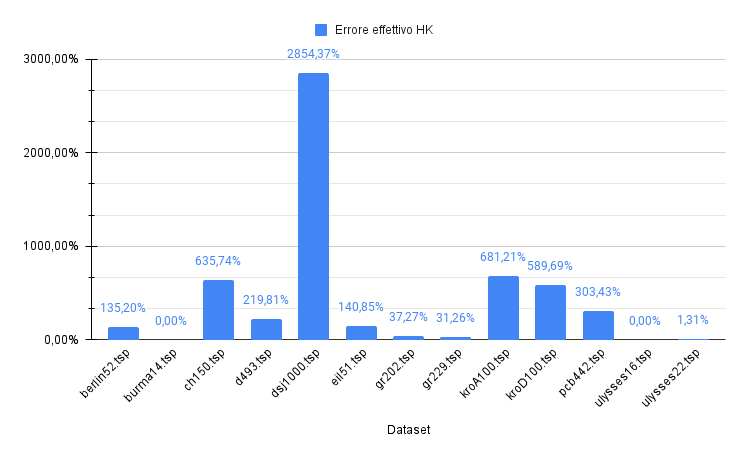
\includegraphics[width=0.85\textwidth]{res/images/errors/hk-effettivo.png}
	\caption{Errore effettivo dei risultati ottenuti con Held-Karp.}
	\label{fig:errors-hk-effettivo}
\end{figure}

\begin{figure}[H]
	\centering
	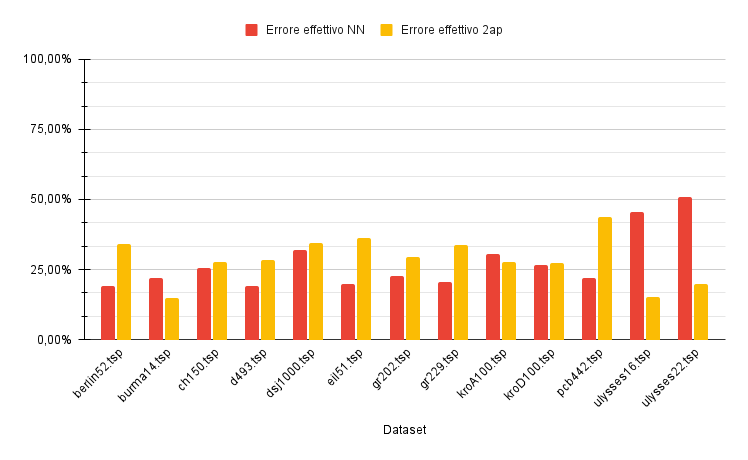
\includegraphics[width=0.85\textwidth]{res/images/errors/approx-effettivo.png}
	\caption{Errore effettivo dei risultati ottenuti con gli algoritmi non esatti.}
	\label{fig:errors-approx-effettivo}
\end{figure}

\begin{figure}[H]
	\centering
	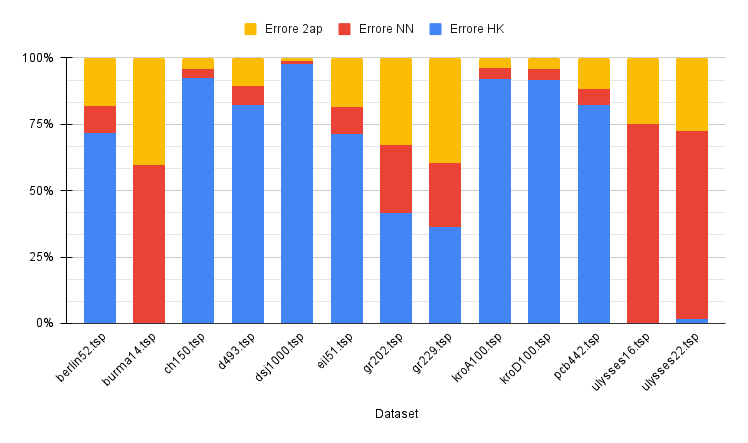
\includegraphics[width=0.85\textwidth]{res/images/errors/all.png}
	\caption{Errori in proporzione per i tre algoritmi.}
	\label{fig:errors-all}
\end{figure}

\begin{figure}[H]
	\centering
	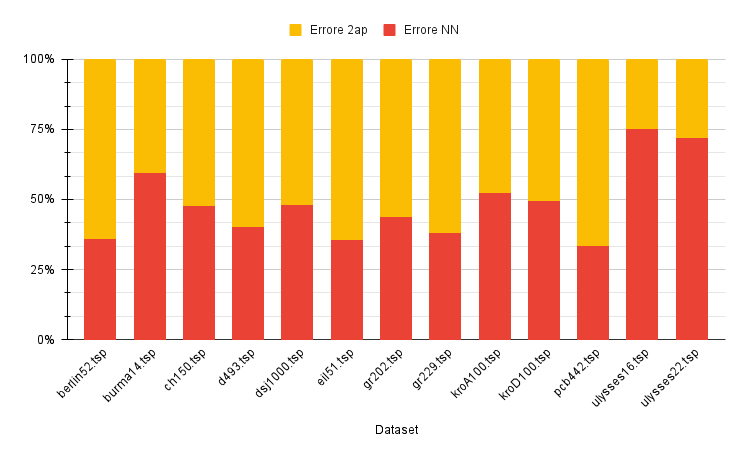
\includegraphics[width=0.85\textwidth]{res/images/errors/approx.png}
	\caption{Errori in proporzione per gli algoritmi non esatti.}
	\label{fig:errors-approx}
\end{figure}

Come si può evincere da questi grafici (fig. \ref{fig:errors-hk-effettivo}, \ref{fig:errors-approx-effettivo}, \ref{fig:errors-all}, \ref{fig:errors-approx}), l'algoritmo nearest neighbor sembra essere, \textit{in media}, più efficiente; ciò non è vero, però, per grafi più piccoli come \textit{burma14}, \textit{ulysses16} e \textit{ulysses22}, in cui l'algoritmo di 2-approssimazione si avvicina decisamente meglio alla soluzione ottima. 
Una possibile ipotesi che abbiamo avanzato nel corso dell'analisi di questi risultati potrebbe ricondursi alla natura \textit{greedy} dell'algoritmo nearest neighbor, che procede con la scelta ottima per ogni vertice incontrato. Pertanto, la potenzialità di questo algoritmo si riflette meglio con grafi di maggior dimensione proprio perché il numero di scelte da effettuare è maggiore e quindi il possibile tasso di errore si riduce in proporzione. Chiaramente questa ipotesi è puramente un'osservazione basata su nostre congetture che sarebbe interessante approfondire. 


\begin{figure}[H]
	\centering
	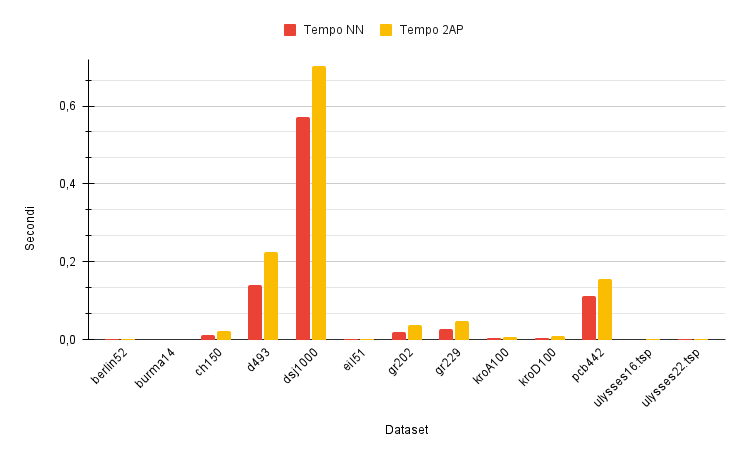
\includegraphics[width=1\textwidth]{res/images/time/time-nn-2ap.png}
	\caption{Tempi effettivi ottenuti con Nearest Neighbor e 2-approssimazione.}
	\label{fig:time-nn-2ap}
\end{figure}

Per quanto riguarda le tempistiche degli algoritmi di approssimazione, si può notare dal grafico \ref{fig:time-nn-2ap} che i tempi di esecuzione dei due algoritmi, anche ripetuti più e più volte, denotano un minore tempo di computazione effettivo per l'algoritmo di Nearest Neighbor, specialmente nei grafi più grandi. 
Analogamente, anche nei grafi di minore dimensione (fig. \ref{fig:time-detail-nn-2ap}) è possibile notare che questo algoritmo è quello che ci impiega meno tempo a livello computazionale, confermandosi quindi il più veloce dei tre. 

\begin{figure}[H]
	\centering
	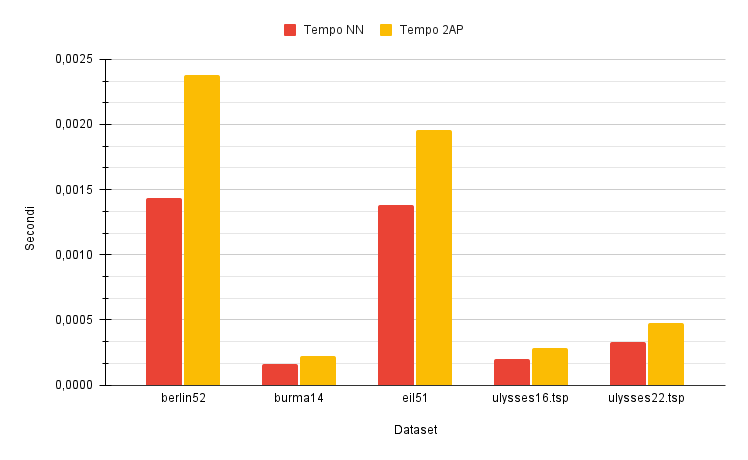
\includegraphics[width=1\textwidth]{res/images/time/time-detail-nn-2ap.png}
	\caption{Dettaglio dei tempi effettivi ottenuti con Nearest Neighbor e 2-approssimazione nei dataset più piccoli.}
	\label{fig:time-detail-nn-2ap}
\end{figure}

Per quanto concerne le tempistiche di Held and Karp, solo due dataset hanno computato il risultato entro tre minuti, mentre uno di questi, \textit{ulysses22}, ci è andato vicino con un errore del 1,31\% (fig. \ref{fig:errors-hk-effettivo}). Altri dataset, come \textit{burma14} e \textit{ulysses16}, hanno completato la computazione e hanno ottenuto in un tempo relativamente basso i risultati, rispettivamente di circa 0.35 e 1.96 secondi.

% Conclusione e sviluppi futuri
\newpage
\section{Conclusione}

% ottimizzazioni su naive molto utili --> risparmio di diverse chiamate a dfs / primi grafi molto veloci quasi quanto UF e prim

Alla fine del lavoro svolto possiamo dire che le ottimizzazioni che sono state implementate per la versione naive dell'algoritmo di Kruskal si sono 
rivelate utili per l'esecuzione dei primi grafi. Infatti,
\begin{enumerate}
    \item Il controllo dei \textit{self-loop} e della presenza o meno dei nodi dell'arco $(u, v)$ hanno permesso di risparmiare diverse chiamate a DFS per il 
    controllo della ciclicità del grafo $G$;
    \item La versione modificata di DFS permette di evitare la visita di tutto il grafo quando non è necessario. È sufficiente controllare che esista un cammino 
    da $u$ a $v$ nella componente connessa di $u$. Se tale cammino non esiste, allora il lato $(u, v)$ farà parte del MST $T$ finale.
\end{enumerate}
Queste ottimizzazioni hanno permesso di ottenere delle performance migliori nel momento in cui l'algoritmo inizia ad analizzare il grafo ricevuto in 
input. È possibile notare che i tempi per Kruskal Naive sono paragonabili ai tempi degli altri due algoritmi per grafi con un piccolo numero di vertici (cfr. \S{4.3}).


% ottimizzazione dello heap per Prim --> risparmio sulla ricerca lineare

In secondo luogo, per quanto riguarda l'implementazione della struttura dati Heap utilizzata per l'algoritmo di Prim abbiamo potuto constatare che l'ottimizzazione integrata attraverso una mappa che permettesse di salvare l'indice di posizione corrente nella lista ausiliaria ha ridotto di gran lunga la durata media dell'algoritmo di Prim, tendendo a essere più simile al tempo medio ottenuto da Kruskal Union Find. Questa miglioria ha permesso di accedere quindi in tempo costante ai singoli elementi della lista rimuovendo la complessità lineare, che precedentemente avrebbe reso computazionalmente più lento di un valore polinomiale l'algoritmo di Prim.


% misurazione più accurate 

Per quanto concerne le misurazioni effettuate abbiamo voluto rendere ciascuna misurazione il più preciso possibile così da ottenere risultati sui tempi medi di esecuzione più attendibili. Difatti, ripetendo l'esecuzione di ciascun grafo con tempo di esecuzione minore al secondo di un fattore \(k\), che rappresenta il numero di ripetizioni da eseguire per rientrare entro il secondo sulla base del tempo per una esecuzione, siamo riusciti ad avere un risultato più comparabile che ci ha permesso di fare dei confronti più interessanti (vedasi i risultati della sezione \S{4). 


% approccio di lavoro incrementale, ossia creo algoritmo, verifico efficacia (3 risultati uguali = risultati corretti), lo ottimizzo
Per quanto concerne il \textit{workflow} adottato all'interno del gruppo, avendo lavorato con un sistema di versionamento siamo riusciti ad organizzarci per realizzare e sviluppare attraverso un approccio incrementale ciascun algoritmo. Inizialmente infatti abbiamo iniziato con lo studiare bene il funzionamento di ogni algoritmo e poi, gradualmente, lo abbiamo implementato partendo dalle strutture dati richieste. Una volta controllato che in tutti e 3 i casi gli algoritmi ottenevano risultati identici sul peso finale degli archi, abbiamo ottimizzato ciascuno di essi limando sulle parti di codice superflue ed applicando delle migliorie in base a quanto il linguaggio Python ha da offrire. Infine, abbiamo voluto anche rendere facilmente utilizzabile l'applicazione finale, così da poter provare diversi dataset in diverse modalità. Per la realizzazione dei grafi, tuttavia, abbiamo preferito raccogliere i risultati e generare i grafici sfruttando Google Colab, la cui logica è stata riportata per completezza all'interno di una cartella del progetto (\textit{graph-generation}).


% tiriamo le somme sui risultati 

In linea di massima siamo stati contenti dei risultati ottenuti sebbene l'uso del linguaggio Python, pur se relativamente semplice, ci è risultato abbastanza disordinato per la mancanza di \textit{strong typing}, cosa che ci ha causato inizialmente diversi rallentamenti nello sviluppo degli algoritmi.
Per concludere, quanto ci è risultato per gli algoritmi è in linea con quanto ci aspettavamo, difatti: 
\begin{itemize}
    \item Kruskal Naive risulta il più lento tra i tre algoritmi e il meno efficiente in termini di tempo medio di esecuzione per grafi con molti nodi;
    \item Kruskal Union Find risulta il più veloce e il più efficiente tra i tre algoritmi, specialmente con grafi di grandi dimensioni;
    \item Prim si può classificare in secondo posto rispetto a Kruskal Union Find, avendo un tempo di esecuzione sufficientemente buono anche per grafi di grandi dimensioni. 
\end{itemize}





% Appendice
\newpage
\begin{appendices}

   \section{Appendice}

\subsection{Risultati output Stoer e Wagner}

\subsection{Risultati output Karger e Stein}

\end{appendices}